% This is samplepaper.tex, a sample chapter demonstrating the
% LLNCS macro package for Springer Computer Science proceedings;
% Version 2.20 of 2017/10/04
%
\documentclass[runningheads]{llncs}
%
\usepackage[a4paper, left=2.5cm, right=2.5cm, top=2.5cm, bottom=2.5cm]{geometry}

\usepackage{mathptmx}   % loads Times New Roman
\usepackage{setspace}   % for interline spacing
\onehalfspacing         % interline spacing of 1.5 in main text, 1 in footnotes 


\usepackage{graphicx}
\usepackage{array}
\usepackage{tabularx} 

% Here, I redefine \tabular to automatically switch to
% \footnotesize within the scope of a tabular environment.
\let\oldtabular\tabular
\renewcommand{\tabular}{\footnotesize\oldtabular}

% Used for displaying a sample figure. If possible, figure files should
% be included in EPS format.
%
% If you use the hyperref package, please uncomment the following line
% to display URLs in blue roman font according to Springer's eBook style:
% \renewcommand\UrlFont{\color{blue}\rmfamily}

\begin{document}
%
\title{The ABC of Software Engineering Research}
%
%\titlerunning{Abbreviated paper title}
% If the paper title is too long for the running head, you can set
% an abbreviated paper title here
%
\author{Faiz Ahmed}
%
%\authorrunning{F. Author et al.}
% First names are abbreviated in the running head.
% If there are more than two authors, 'et al.' is used.
%
\institute{Christian-Albrecht University of Kiel, Germany
\\
\email{stu225473@mail.uni-kiel.de}}
%
\maketitle              % typeset the header of the contribution
%
\begin{abstract}
This paper presents the ABC framework, which is adapted from the taxonomy developed by McGrath and his colleagues in the social
sciences, and seeks to provide guidance to help researchers select an appropriate research strategy that aligns with the goals of their research. The ABC framework contributes to the discourse on research methodology in software engineering by offering an alternative, holistic view that positions eight archetypal research strategies. I will discuss metaphors for each strategy and their inherent limitations and potential strengths. 

\keywords{SE  \and Extreme Programming \and Global Software Engineering.}
\end{abstract}
%
%
%
\section{Introduction}
\label{section1}
The term ABC refers to the research goal that strives for generalizability over Actors(A) and precise measurement of their Behavior (B), in a realistic Context (C). The ABC framework uses two dimensions widely considered to be key in research design: the level of obtrusiveness of the research and the generalizability of research findings. 

\section{Dimensions of Research Strategies}
\label{section2}
Two important dimensions of a research strategy are the level of obtrusiveness and generalizability. These two dimensions are the axes in the ABC framework.

\subsection{Obtrusiveness}
The first dimension is concerned with how \emph{obtrusive} the research is: to what extent does a researcher “intrude” on the research setting, or simply make observations in an unobtrusive way. Researchers who wish to exert more control in a research study usually have to intrude in the research setting, for example, to manipulate some variables. Several authors have
argued that the level of control that a researcher can exert while conducting a study is a key concern. One concern often raised in the context of qualitative methods
such as ethnographic and case study research is a lack of control. Parnas lamented the lack of
experimental design in current empirical software development research and how observations
from a small number of “uncontrolled case studies” do not contribute to scientific knowledge ~\cite{ref_article15} .

\subsection{Generalizability}
A second key concern that authors have expressed is the level of generalizability of research findings. This has been a recurring concern in software engineering research, in particular in the context of case studies captured succinctly by one referee: “Case study reports are [ . . . ] limited, because they report a single case.”

\section{THE ABC FRAMEWORK FOR RESEARCH STRATEGIES}
\label{section3}
This section presents a framework that provides a holistic overview of eight different research
strategies. The framework, which we have termed the ABC framework (Figure ~\ref{fig1}), was originally
devised by McGrath and his colleagues for the social sciences \cite{ref_article1,ref_article2,ref_article3,ref_article4} .

\begin{figure}
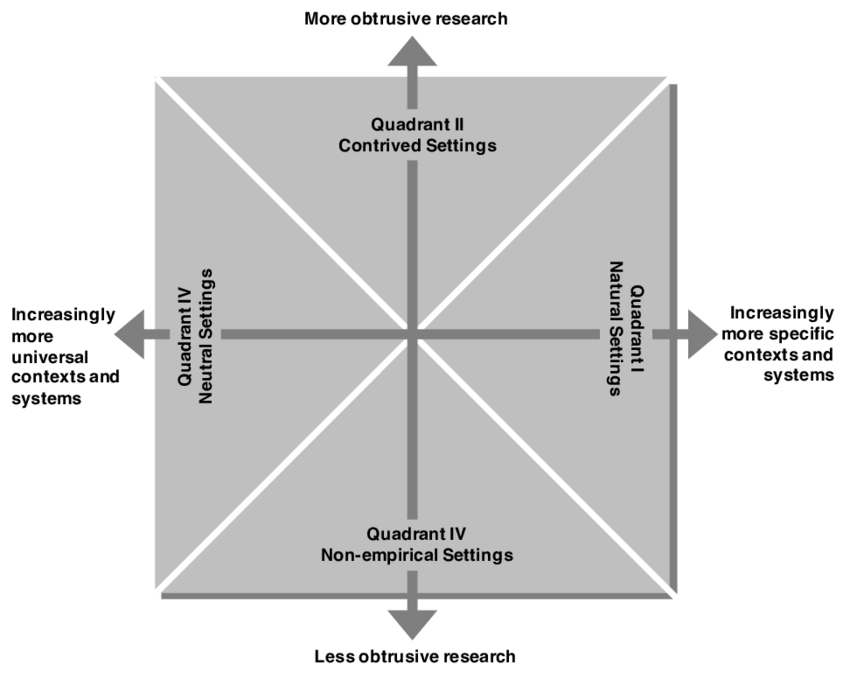
\includegraphics[width=\textwidth]{fig1.png}
\caption{The ABC framework: eight research strategies as categories of research methods for software engi-neering (adapted from Runkel and McGrath ~\cite{ref_article5}). Quadrants I to IV represent different research settings} \label{fig1}
\end{figure}
\subsection{Field Studies}
\emph{Field study} refers to any research conducted in a specific, real-world setting to study a specific software engineering phenomenon. The field study strategy is located in Quadrant I (Figure 1), representing natural settings. Field studies are unobtrusive in that a researcher does not actively control or change any parameters or variables. That is, there is no deliberate modification of the research setting.
\\
One example of a field study in SE is an ethnographic study of XP (Extreme Programming) by
Sharp et al ~\cite{ref_article6} . This study did not aim to “control” any variables, nor to change anything in the case study setting. Rather, the authors stated that their “motivation is to gain insight into the culture and community of an agile method.” The metaphor we chose for field studies is the \emph{jungle}. 

\subsection{Field Experiments}
A \emph{field experiment} refers to an experimental study conducted in a natural setting with a high degree of realism (similar to a field study), but in this strategy the researcher manipulates some properties or variables in the research setting so as to observe an effect of some kind—this manipulation educes the level of realism compared to a field study. The realistic research setting exists independent of the researcher, which distinguishes it from the contrived research setting in a laboratory experiment. Common settings for field experiments in SE include a specific software development organization or team or a deployed production system.
\\
They suggest a \emph{nature reserve} as a metaphor for a field experiment setting. In a nature reserve, flora and fauna can still thrive as normal, but the reserve facilitates the conduct of research, for example, by placing fences so as to separate the wildlife into different treatment groups and evaluate the effects of those treatments.
\subsection{Experimental Simulations}
The \emph{experimental simulation} strategy is one of two strategies in Quadrant II—the quadrant that represents contrived research settings. In an experimental simulation, the behaviors of actors (e.g., developers, users, or software systems) that a researcher aims to observe and measure are natu-ral.
\\
I borrow Runkel and McGrath’s metaphor, who compared an experimental simulation to a
greenhouse ~\cite{ref_article6}. A greenhouse is built to simulate a certain setting, optimized for certain characteristics, for example, to grow fruits that require much sunlight and high temperatures, which otherwise could not be grown in cold climates.

\subsection{Laboratory Experiments}

The \emph{laboratory experiment} is the second strategy in Quadrant II. It differs from field experiments, which are positioned in Quadrant I and thus study phenomena in their natural context, whereas laboratory experiments are set in a contrived setting. A laboratory experiment is characterized by a high potential to neutralize any confounding factors and extraneous conditions ~\cite{ref_article6}. Consequently, laboratory experiments allow a researcher to exercise maximum precision of measurement of behavior on the studied object—this is indicated by the Quadrant II in Figure ~\ref{fig1}.
\\
A useful metaphor for laboratory experiment is a \emph{test tube}, which Runkel and McGrath ~\cite{ref_article6} used to set it clearly apart from the greenhouse (experimental simulation, representing a more continuous flow of events) and nature reserve (field experiment)

\subsection{Judgment Studies}
A \emph{judgment study} involves gathering empirical data from a group of participants who are asked to judge or rate behaviors, to respond to a request or “stimulus” offered by a researcher, or to discuss a given topic of interest. Judgment studies rely on systematic sampling rather than representative sampling and should involve experts, appropriately informed to respond to a certain question or stimulus. The goal of a judgment study is to seek generalizability over the responses, rather than generalizability to a population of actors.
\\
I liken a judgment study to a \emph{courtroom}, in which a panel of participants (the jury) are carefully and systematically selected. In a courtroom, evidence is presented (a \emph{stimulus}) and eventually the jury returns a verdict.

\subsection{Sample Studies}
Also in Quadrant III is the \emph{sample study} strategy, which aims to achieve generalizability over a certain population of \emph{actors}, whether these are software professionals, software systems, or artifacts of the development process. The sample study is one of two strategies with the potential to maximize generalizability to a population—this is indicated by the Quadrant III in Figure ~\ref{fig1}.

A metaphor for the sample study strategy is a \emph{referendum} (though we admit this only suggests samples of human participants, not development artifacts). In a referendum, usually a limited set of questions is presented to a large group of people, who are invited to respond—typically, only a sample actually responds.

\subsection{Formal Theory}
\emph{Formal theory} is one of two strategies in Quadrant IV that have no empirical setting. Formal theory\footnote{Not to be confused with formal methods that are used, for example, to develop formal program specifications.} is a strategy that aims at a high level of universality so that the resulting theory or framework can be applied under a wide array of circumstances, although most theories have boundaries outside of which they do not apply \cite{ref_article7}.
\\
As a metaphor, we propose that developing formal theory is akin to solving a \emph{jigsaw puzzle}. Solving a jigsaw puzzle can be done as a solitary or team effort, it happens in a nonempirical context(e.g., at a large table to fit all the pieces), and the goal is to “fit” all pieces together.

\subsection{Computer Simulations}
The eighth research strategy is \emph{computer simulation}, also positioned in Quadrant IV. The goal of a computer simulation is to create a symbolic replica of a certain type of concrete system that can be executed by a computer \cite{ref_article6}. In a computer simulation of a real-world phenomenon or setting, everything is represented symbolically and created artificially.
\\
As a metaphor, we liken a computer simulation to a \emph{forecasting system}, such as those used in weather prediction, which employ complex mathematical models of the atmosphere and oceans.Such systems are programmed to do a very specific thing based on a set of preprogrammed rules.

\section{APPLICABILITY OF THE ABC FRAMEWORK TO SOFTWARE
ENGINEERING RESEARCH}
\label{section4}
To illustrate the use of different research strategies in software engineering research, we present examples from two different research areas: Global Software Engineering (GSE) and Requirements Engineering (RE). Table \ref{tab1}, discusses examples of Different Research Strategies Used in Global Software Engineering Research.

\subsection{Research Strategies in Global Software Engineering Research}
GSE has been actively studied since the 1990s, and research has focused primarily on the challenges associated with distributed development, whether as a result of offshoring or outsourcing strategies.

\begin{table}
\caption{Examples of Different Research Strategies Used in Global Software Engineering Research.}\label{tab1}
\begin{tabularx}{1\textwidth} { 
   >{\raggedright\arraybackslash}X 
   >{\raggedright\arraybackslash}X 
   >{\raggedright\arraybackslash}X 
   >{\raggedright\arraybackslash}X
   >{\raggedright\arraybackslash}X
   >{\raggedright\arraybackslash}X }
\hline
Strategy & Authors &  Objective &  Study Setting &  Study Procedure & Findings
\\
\hline
Field Study &  
Herbsleb and Grinter 1999 \cite{ref_proc1} & 
To understand why geographically distributed development is difficult to coordinate. & 
\emph{Natural}: Two ocations of a division of Lucent Technologies &
18 interviews, archival sources, documents.&
Coordination mechanisms; barriers to informal communication; 
\\
\hline
Experimental Simulation & 

Bos et al.2004 \cite{ref_proc3} &

To investigate the impact of colocation, coaching. & 

\emph{Natural}: Alcatel’s Switching and Routing business unit.  & 
Comparison of inspections in colocated and distributed teams;&
Colocating peer reviews improves defect detection; 
\\
\hline
Experimental Simulation &
Bos et al. 2004 \cite{ref_proc2} &

To study the effect of
colocation, the
presence of multiple
sites within a large
company. &

Contrived: online
multiplayer game (the
Shape Factory
simulation
environment).& 

13 simulation sessions
with 5 rounds each;
10 players per session,
130 participants in total. &

Colocated participants
collaborated more with each
other than with
telecommuters. 
\\
\hline
Laboratory Experiment & 
Babar et al.2008 ~\cite{ref_article10} &
To study the impact of groupware support on the quality of software architecture. &
Contrived: experimental tasks part of assessed course tasks. &
Controlled experiment, AB/BA crossover design; 32 teams of 3 participants. & 
Quality of deliverables from the distributed meeting groups was good.
\\
\hline
Judgment Study &
Iacovou and Nakatsu 2008 \cite{ref_book1} &
To investigate risk factors for offshore-outsourcing software development. &
Neutral: systematically selected panel of experts at a variety of organizations. &

Delphi study, 15 experts, 3 rounds: identification; rating; &
25 risk factors that could influence the success of an offshore-outsourced project.
\\
\hline
Sample Study & 
Ma et al.2008 ~\cite{ref_proc4} &
To investigate 3 issues in software development by Chinese software suppliers. &
Neutral: questionnaire sent out to companies by email.&
Random sample of 2,000 from a database of approx. &
Language not a major obstacle; email used for development issues. 
\\
\hline
Formal Theory &
Espinosa and Carmel 2003 ~\cite{ref_proc5} &
To develop a conceptual foundation for future research on GSE. &
Nonempirical: desk research without any direct empirical observations & 
Theorizing and conceptualization based on Coordination Theory &
A model of coordination costs due to time differences in dispersed software teams.
\\
\hline
Computer Simulation & 
Setamanit et al. 2007 ~\cite{ref_article8,ref_article9} &
To evaluate the choice of task allocation strategy. &
Nonempirical: GSD simulator with which the researchers can model several factors. & For each of 3 strategies: 5 replications for each design point. & 
1,920 runs in total. Increasing overlap of work hours contributes to shorter.
\\
\hline
\end{tabularx}
\end{table}


\subsection{Research Strategies in Requirements Engineering Research}
In this section, we illustrate the different research strategies with a second research area: Requirements Engineering. RE has long been one of the core areas within software engineering research, with a first special issue in IEEE Transactions on Software Engineering in 1977 ~\cite{ref_article11}. The following Table \ref{tab2} shows the Distribution of Research Strategies of the Analyzed Sample.

\begin{table}
\caption{Distribution of Research Strategies of the Analyzed Sample}\label{tab2}
\begin{center}
\begin{tabular}{ l c } 
\hline
Strategy & Counts 
\\
\hline
Field Study &  10
\\
Experimental Simulation & 0
\\
Experimental Simulation & 4
\\
Laboratory Experiment & 30
\\
Judgment Study & 3
\\
Sample Study & 38
\\
Formal Theory & 0
\\
Computer Simulation & 0
\\
\hline
\end{tabular}
\end{center}
\end{table}

\subsection{Analysis of a Sample of Studies}
Our analysis above is based on a convenience sample; we selected studies that exemplify the eight research strategies. In order to demonstrate a wider applicability of the framework, we analyzed all articles published in 2017 in Springer’s Empirical Software Engineering journal.

\section{DISCUSSION AND CONCLUSION}
\label{section5}
\subsection{Metaphors and Research Settings in Software Engineering}
or each research strategy, we presented a metaphor representing that strategy within its research setting (see Section ~\ref{section3} ), some of which were proposed by others ~\cite{ref_article4,ref_article12}.

\subsection{The A, B, and C of Software Engineering Research}
The ABC framework positions eight archetypal research strategies that SE researchers can use,in particular for what we have termed knowledge-seeking studies (see Section 1). The framework is based on earlier work in the social sciences ~\cite{ref_article1,ref_article2,ref_article3,ref_article4,ref_article5}, which we have adapted and operationalized for a software engineering context.

\subsection{Limitations of the ABC Framework}
Given the socio-technical nature of the software engineering field, we argue that the framework, though rooted in the social sciences, is also useful to SE research. We have demonstrated the fit of the ABC framework on two worked examples in Section 4. In addition, we analyzed a sample of 75 articles published in 2017 in Empirical Software Engineering; we classi-fied all knowledge-seeking studies using the ABC framework. Notwithstanding the fit of the ABC framework, some limitations of the framework should be borne in mind.

\subsection{Conclusion}
The software engineering research community has made considerable progress in terms of the quality of studies that seek knowledge and understanding. Over the last several decades, the community has reflected on the way it conducts research and the methods to do that research. There are numerous guidelines for employing specific methods, and the variety of research methods has increased without a doubt. Nevertheless, there is still some confusion about terminology, and the
various overviews of research methods are a“mixed bag” in that the various methods identified have not been carefully positioned in relation to one another. A holistic view of the landscape of research strategies to generate new knowledge and understanding has been missing so far in the SE research community. In this article, we adopt a framework from the social sciences that we have labeled the ABC framework—as such, it contributes to the literature on research methodology for
software engineering.
%
% ---- Bibliography ----
%
% BibTeX users should specify bibliography style 'splncs04'.
% References will then be sorted and formatted in the correct style.
%
% \bibliographystyle{splncs04}
% \bibliography{mybibliography}
%
\begin{thebibliography}{8}

\bibitem{ref_article1}
J. E. McGrath. 1964. Towards a “Theory of Method” for research on organizations. In New Perspectives in Organization Research, W. Cooper, H. Leavitt, and M. Shelly (Eds.). John Wiley \& Sons, New York, 533–556

\bibitem{ref_article2}
J. E. McGrath. 1984. Groups: Interaction and Performance. Prentice-Hall.

\bibitem{ref_article3}
J. E. McGrath. 1994. Methodology matters: Doing research in the behavioral and social sciences. In Readings in Human-Computer Interaction: Toward the Year 2000, Ronald M. Baecker (Ed.). Morgan Kaufmann, 152–169.

\bibitem{ref_article4}
P. J. Runkel and J. E. McGrath. 1972. Research on Human Behavior: A Systematic Guide to Method. Holt, Rinehart and
Winston.

\bibitem{ref_article5}
P. J. Runkel and J. E. McGrath. 1972. Research on Human Behavior: A Systematic Guide to Method. Holt, Rinehart and
Winston

\bibitem{ref_article6}
H. Sharp and H. Robinson. 2004. An ethnographic study of XP practice. Empir. Software Eng. 9, 4 (2004), 353–375

\bibitem{ref_article7}
K. Stol and B. Fitzgerald. 2015. Theory-oriented software engineering. Sci. Computer Program. 101 (2015), 79–98

\bibitem{ref_proc1}
J. D. Herbsleb and R. E. Grinter. 1999. Splitting the organization and integrating the code: Conway’s law revisited. In Proc. International Conference on Software Engineering. 85–95.

\bibitem{ref_proc2}
N. Bos, N. Sadat Shami, J. S. Olson, A. Cheshin, and N. Nan. 2004. In-group/out-group effects in distributed teams:
An experimental simulation. In Proc. International Conference on Computer-Supported Cooperative Work and Social
Computing (CSCW’04). ACM, New York, 429–436.

\bibitem{ref_proc3}
C. Ebert, C. H. Parro, R. Suttels, and H. Kolarczyk. 2001. Better validation in a world-wide development environment.
In Proc. 7th International Software Metrics Symposium (METRICS’01).

\bibitem{ref_book1}
C. L. Iacovou and R. Nakatsu. 2008. A risk profile of offshore-outsourced development projects. Commun. ACM 51,
6 (2008), 89–94.

\bibitem{ref_proc4}
J. Ma, J. Li, W. Chen, R. Conradi, J. Ji, and C. Liu. 2008. A state-of-the-practice study on communication and coordination between Chinese software suppliers and their global outsourcers. Software Process Improve. Pract. 13, 3
(2008), 233–247.

\bibitem{ref_proc5}
J. A. Espinosa and E. Carmel. 2003. The impact of time separation on coordination in global software teams: A
conceptual foundation. Software Process. Improve. Pract. 8, 4 (2003), 249–266

\bibitem{ref_article8}
D. Raffo and S.-O. Setamanit. 2005. A simulation model for global software development project. In Proc. 6th Inter-
national Workshop on Software Process Simulation and Modeling (ProSim’05). Fraunhofer IRB Verlag.

\bibitem{ref_article9}
S.-O. Setamanit, W. Wakeland, and D. Raffo. 2007. Using simulation to evaluate global software development task
allocation strategies. Software Process Improve. Pract. 12 (2007), 491–503.

\bibitem{ref_article10}
M. A. Babar, B. Kitchenham, and R. Jeffery. 2008. Comparing distributed and face-to-face meetings for software
architecture evaluation: A controlled experiment. Empir. Software Eng. 13, 1 (2008), 39–62.

\bibitem{ref_article11}
D. T. Ross. 1977. Guest editorial: Reflections on requirements. IEEE Trans. Software Eng. 3, 1 (1977), 2–5.

\bibitem{ref_article12}
E. R. McLean. 1973. Comments on empirical studies of management information systems by Richard L. Van Horn.
Data Base 5, 2 (1973), 181–182.

\bibitem{ref_article13}
Stol, K.-J. and Fitzgerald, B. (2018) 'The ABC of Software Engineering Research', ACM Transactions on Software Engineering and Methodology, 27(3), 11 (51 pp). doi: 10.1145/3241743
%\bibitem{ref_url1}
%LNCS Homepage, \url{http://www.springer.com/lncs}. Last accessed 4 Oct 2017
\bibitem{ref_article14}
Steve Easterbrook, Janice Singer, Margaret-Anne Storey, and Daniela Damian. Selecting Empirical Methods for Software Engineering Research

\bibitem{ref_article15}
D. L. Parnas. 2009. Point/counterpoint: Empirical research in software engineering: A critical view. IEEE Software
26, 6 (2009), 56–59.

\end{thebibliography}
\end{document}
